\documentclass[11pt,fleqn, openany]{book} % Default font size and left-justified equations

%%%%%%%%%%%%%%%%%%%%%%%%%%%%%%%%%%%%%%%%%
% The Legrand Orange Book
% Structural Definitions File
% Version 2.1 (26/09/2018)
%
% Original author:
% Mathias Legrand (legrand.mathias@gmail.com) with modifications by:
% Vel (vel@latextemplates.com)
% 
% This file was downloaded from:
% http://www.LaTeXTemplates.com
%
% License:
% CC BY-NC-SA 3.0 (http://creativecommons.org/licenses/by-nc-sa/3.0/)
%
%%%%%%%%%%%%%%%%%%%%%%%%%%%%%%%%%%%%%%%%%

%----------------------------------------------------------------------------------------
%	VARIOUS REQUIRED PACKAGES AND CONFIGURATIONS
%----------------------------------------------------------------------------------------

\usepackage[table]{xcolor}

\usepackage{graphicx}
\usepackage{tabularx} % Required for including pictures
\usepackage{pgf,tikz,tkz-tab,eurosym,yhmath, stmaryrd}
\usepackage{pgfplots}
\usepackage{mathrsfs}
\usetikzlibrary{patterns}
\usetikzlibrary{trees}
\graphicspath{{../../Pictures/}}
\usepackage{multicol} 


\usepackage[english]{babel} % English language/hyphenation
\usepackage{icomma}
\usepackage{enumitem} % Customize lists
\setlist{nolistsep, nosep, nolistsep} % Reduce spacing between bullet points and numbered lists

\usepackage{booktabs} % Required for nicer horizontal rules in tables

 % Required for specifying colors by name


\definecolor{ocre}{RGB}{243,102,25} % Define the orange color used for highlighting throughout the book

\usepackage{listings}

\definecolor{codegreen}{rgb}{0,0.6,0}
\definecolor{codegray}{rgb}{0.5,0.5,0.5}
\definecolor{codepurple}{rgb}{0.58,0,0.82}
\definecolor{backcolour}{rgb}{0.95,0.95,0.92}

\lstdefinestyle{mystyle}{
    backgroundcolor=\color{backcolour},   
    commentstyle=\color{codegreen},
    keywordstyle=\color{magenta},
    numberstyle=\tiny\color{codegray},
    stringstyle=\color{codepurple},
    basicstyle=\ttfamily\footnotesize,
    breakatwhitespace=false,         
    breaklines=true,                 
    captionpos=b,                    
    keepspaces=true,                 
    numbers=left,                    
    numbersep=5pt,                  
    showspaces=false,                
    showstringspaces=false,
    showtabs=false,                  
    tabsize=2
}

\lstset{style=mystyle}

%----------------------------------------------------------------------------------------
% Paramétrage XSIM
%----------------------------------------------------------------------------------------

\usepackage[no-files]{xsim}


\DeclareExerciseEnvironmentTemplate{myex}{%
    \textbf{%
      \hypertarget{ex:\ExerciseID}{\sffamily{\ensuremath{\blacktriangleright}} Exercice \GetExerciseProperty{counter} \GetExerciseProperty{subtitle} --}
      \hyperlink{sol:\ExerciseID}{Voir le corrigé}%
    }\par
}{\par\smallskip}

\DeclareExerciseEnvironmentTemplate{mysol}{%
    \textbf{%
      \hypertarget{sol:\ExerciseID}{\sffamily{\ensuremath{\blacktriangleright}} Correction \GetExerciseProperty{counter} --}
      \hyperlink{ex:\ExerciseID}{Voir l'énoncé}%
    }\par
}{\par\medskip}

\xsimsetup{
  exercise/template = myex ,
  solution/template = mysol 
}

%Collection exercices

\DeclareExerciseTagging{topic}

\xsimsetup{collect}

%----------------------------------------------------------------------------------------
% SYMBOLES
%----------------------------------------------------------------------------------------

\newcommand\imCMsym[4][\mathord]{%
  \DeclareFontFamily{U} {#2}{}
  \DeclareFontShape{U}{#2}{m}{n}{
    <-6> #25
    <6-7> #26
    <7-8> #27
    <8-9> #28
    <9-10> #29
    <10-12> #210
    <12-> #212}{}
  \DeclareSymbolFont{CM#2} {U} {#2}{m}{n}
  \DeclareMathSymbol{#4}{#1}{CM#2}{#3}
}
\newcommand\alsoimCMsym[4][\mathord]{\DeclareMathSymbol{#4}{#1}{CM#2}{#3}}

\imCMsym{cmmi}{124}{\CMjmath}

\newcommand{\Oij}{(O\,;\,\vec{\imath}\,,\, \vec{\CMjmath} )}
\newcommand{\Oijk}{(O\,;\,\vec{\imath}\,,\, \vec{\CMjmath}\,,\,\vec{k})}

\newcommand\e{\mathrm{e}}
\newcommand\R{\mathbb{R}}
\newcommand\N{\mathbb{N}}


%----------------------------------------------------------------------------------------
%	MARGINS
%----------------------------------------------------------------------------------------

\usepackage{geometry} % Required for adjusting page dimensions and margins

\geometry{
	paper=a4paper, % Paper size, change to letterpaper for US letter size
	top=3cm, % Top margin
	bottom=3cm, % Bottom margin
	left=2cm, % Left margin
	right=2cm, % Right margin
	headheight=14pt, % Header height
	footskip=1.4cm, % Space from the bottom margin to the baseline of the footer
	headsep=10pt, % Space from the top margin to the baseline of the header
	%showframe, % Uncomment to show how the type block is set on the page
}

\setlength{\parindent}{0pt}
\parskip=5pt



%----------------------------------------------------------------------------------------
%	FONTS
%----------------------------------------------------------------------------------------

\usepackage{avant} % Use the Avantgarde font for headings
\usepackage{times} % Use the Times font for headings
\usepackage{mathptmx} % Use the Adobe Times Roman as the default text font together with math symbols from the Sym­bol, Chancery and Com­puter Modern fonts

%\usepackage{microtype} % Slightly tweak font spacing for aesthetics
%\usepackage[utf8]{inputenc} % Required for including letters with accents
\usepackage[T1]{fontenc} % Use 8-bit encoding that has 256 glyphs

%----------------------------------------------------------------------------------------
%	BIBLIOGRAPHY AND INDEX
%----------------------------------------------------------------------------------------

\usepackage[style=numeric,citestyle=numeric,sorting=nyt,sortcites=true,autopunct=true,babel=hyphen,hyperref=true,abbreviate=false,backref=true,backend=biber]{biblatex}
\addbibresource{bibliography.bib} % BibTeX bibliography file
\defbibheading{bibempty}{}

\usepackage{calc} % For simpler calculation - used for spacing the index letter headings correctly
\usepackage{makeidx} % Required to make an index
\makeindex % Tells LaTeX to create the files required for indexing

%----------------------------------------------------------------------------------------
%	MAIN TABLE OF CONTENTS
%----------------------------------------------------------------------------------------

\usepackage{titletoc} % Required for manipulating the table of contents

\contentsmargin{0cm} % Removes the default margin

% Part text styling (this is mostly taken care of in the PART HEADINGS section of this file)
\titlecontents{part}
	[0cm] % Left indentation
	{\addvspace{20pt}\bfseries} % Spacing and font options for parts
	{}
	{}
	{}

% Chapter text styling
\titlecontents{chapter}
	[1.25cm] % Left indentation
	{\addvspace{12pt}\large\sffamily\bfseries} % Spacing and font options for chapters
	{\color{ocre!60}\contentslabel[\Large\thecontentslabel]{1.25cm}\color{ocre}} % Formatting of numbered sections of this type
	{\color{ocre}} % Formatting of numberless sections of this type
	{\color{ocre!60}\normalsize\;\titlerule*[.5pc]{.}\;\thecontentspage} % Formatting of the filler to the right of the heading and the page number

% Section text styling
\titlecontents{section}
	[1.25cm] % Left indentation
	{\addvspace{3pt}\sffamily\bfseries} % Spacing and font options for sections
	{\contentslabel[\thecontentslabel]{1.25cm}} % Formatting of numbered sections of this type
	{} % Formatting of numberless sections of this type
	{\hfill\color{black}\thecontentspage} % Formatting of the filler to the right of the heading and the page number

% Subsection text styling
\titlecontents{subsection}
	[1.25cm] % Left indentation
	{\addvspace{1pt}\sffamily\small} % Spacing and font options for subsections
	{\contentslabel[\thecontentslabel]{1.25cm}} % Formatting of numbered sections of this type
	{} % Formatting of numberless sections of this type
	{\ \titlerule*[.5pc]{.}\;\thecontentspage} % Formatting of the filler to the right of the heading and the page number

% Figure text styling
\titlecontents{figure}
	[1.25cm] % Left indentation
	{\addvspace{1pt}\sffamily\small} % Spacing and font options for figures
	{\thecontentslabel\hspace*{1em}} % Formatting of numbered sections of this type
	{} % Formatting of numberless sections of this type
	{\ \titlerule*[.5pc]{.}\;\thecontentspage} % Formatting of the filler to the right of the heading and the page number

% Table text styling
\titlecontents{table}
	[1.25cm] % Left indentation
	{\addvspace{1pt}\sffamily\small} % Spacing and font options for tables
	{\thecontentslabel\hspace*{1em}} % Formatting of numbered sections of this type
	{} % Formatting of numberless sections of this type
	{\ \titlerule*[.5pc]{.}\;\thecontentspage} % Formatting of the filler to the right of the heading and the page number

%----------------------------------------------------------------------------------------
%	MINI TABLE OF CONTENTS IN PART HEADS
%----------------------------------------------------------------------------------------

% Chapter text styling
\titlecontents{lchapter}
	[0em] % Left indentation
	{\addvspace{15pt}\large\sffamily\bfseries} % Spacing and font options for chapters
	{\color{ocre}\contentslabel[\Large\thecontentslabel]{1.25cm}\color{ocre}} % Chapter number
	{}  
	{\color{ocre}\normalsize\sffamily\bfseries\;\titlerule*[.5pc]{.}\;\thecontentspage} % Page number

% Section text styling
\titlecontents{lsection}
	[0em] % Left indentation
	{\sffamily\small} % Spacing and font options for sections
	{\contentslabel[\thecontentslabel]{1.25cm}} % Section number
	{}
	{}

% Subsection text styling (note these aren't shown by default, display them by searchings this file for tocdepth and reading the commented text)
\titlecontents{lsubsection}
	[.5em] % Left indentation
	{\sffamily\footnotesize} % Spacing and font options for subsections
	{\contentslabel[\thecontentslabel]{1.25cm}}
	{}
	{}

%----------------------------------------------------------------------------------------
%	HEADERS AND FOOTERS
%----------------------------------------------------------------------------------------


\usepackage{fancyhdr} % Required for header and footer configuration

\pagestyle{fancy}
\renewcommand{\chaptermark}[1]{\markboth{\sffamily\normalsize\bfseries\ \thechapter.\ #1}{}} % Chapter text font settings
\renewcommand{\sectionmark}[1]{\markright{\sffamily\normalsize\thesection\hspace{5pt}#1}{}} % Section text font settings
\fancyhf{} \fancyhead[LE,RO]{\sffamily\normalsize\thepage} % Font setting for the page number in the header
\fancyhead[LO]{\rightmark} % Print the nearest section name on the left side of odd pages
\fancyhead[RE]{\leftmark} % Print the current chapter name on the right side of even pages

\fancyfoot[L]{Jason LAPEYRONNIE}
\fancyfoot[R]{\href{http://mathoutils.fr}{http://mathoutils.fr}} % Uncomment to include a footer

\renewcommand{\headrulewidth}{0.5pt} % Thickness of the rule under the header
\renewcommand{\footrulewidth}{0.5pt} % Thickness of the rule under the header

\fancypagestyle{plain}{% Style for when a plain pagestyle is specified
	\fancyhead{}\renewcommand{\headrulewidth}{0pt}%
}

% Removes the header from odd empty pages at the end of chapters
\makeatletter
\renewcommand{\cleardoublepage}{
\clearpage\ifodd\c@page\else
\hbox{}
\vspace*{\fill}
\thispagestyle{empty}
\newpage
\fi}

%----------------------------------------------------------------------------------------
%	THEOREM STYLES
%----------------------------------------------------------------------------------------

\usepackage{amsmath,amsfonts,amssymb,amsthm} % For math equations, theorems, symbols, etc

\newcommand{\intoo}[2]{\mathopen{]}#1\,;#2\mathclose{[}}
\newcommand{\ud}{\mathop{\mathrm{{}d}}\mathopen{}}
\newcommand{\intff}[2]{\mathopen{[}#1\,;#2\mathclose{]}}
\renewcommand{\qedsymbol}{$\blacksquare$}
\newtheorem{notation}{Notation}[section]

% Boxed/framed environments
\newtheoremstyle{ocrenumbox}% Theorem style name
{0pt}% Space above
{0pt}% Space below
{\normalfont}% Body font
{}% Indent amount
{\small\bf\sffamily\color{ocre}}% Theorem head font
{\;:\;}% Punctuation after theorem head
{0.25em}% Space after theorem head
{\small\sffamily\color{ocre}\thmname{#1}\nobreakspace\thmnumber{\@ifnotempty{#1}{}\@upn{#2}}% Theorem text (e.g. Theorem 2.1)
\thmnote{\nobreakspace\the\thm@notefont\sffamily\bfseries\color{black}---\nobreakspace#3}} % Optional theorem note

\newtheoremstyle{blacknumex}% Theorem style name
{5pt}% Space above
{10pt}% Space below
{\normalfont}% Body font
{} % Indent amount
{\small\bf\sffamily}% Theorem head font
{\;:\;}% Punctuation after theorem head
{0.25em}% Space after theorem head
{\small\sffamily{\tiny\ensuremath{\blacksquare}}\nobreakspace\thmname{#1}\nobreakspace\thmnumber{\@ifnotempty{#1}{}\@upn{#2}}% Theorem text (e.g. Theorem 2.1)
\thmnote{\nobreakspace\the\thm@notefont\sffamily\bfseries---\nobreakspace#3}}% Optional theorem note

\newtheoremstyle{blacknumexo}% Theorem style name
{15pt}% Space above
{10pt}% Space below
{\normalfont}% Body font
{} % Indent amount
{\small\bf\sffamily}% Theorem head font
{}% Punctuation after theorem head
{0.5em}% Space after theorem head
{\small\sffamily{\ensuremath{\blacktriangleright}}\nobreakspace\thmname{#1}\nobreakspace\thmnumber{\@ifnotempty{#1}{}\@upn{#2}}% Theorem text (e.g. Theorem 2.1)
\thmnote{\nobreakspace\the\thm@notefont\sffamily\bfseries---\nobreakspace#3} \\}% Optional theorem note



\newtheoremstyle{blacknumbox} % Theorem style name
{0pt}% Space above
{5pt}% Space below
{}% Body font
{}% Indent amount
{\large\bf\sffamily}% Theorem head font
{\;:\;}% Punctuation after theorem head
{0.25em}% Space after theorem head
{\small\sffamily\thmname{#1}\nobreakspace\thmnumber{\@ifnotempty{#1}{}\@upn{#2}}% Theorem text (e.g. Theorem 2.1)
\thmnote{\nobreakspace\the\thm@notefont\sffamily\bfseries---\nobreakspace#3}}% Optional theorem note

% Non-boxed/non-framed environments
\newtheoremstyle{ocrenum}% Theorem style name
{5pt}% Space above
{5pt}% Space below
{\normalfont}% Body font
{}% Indent amount
{\small\bf\sffamily\color{ocre}}% Theorem head font
{\;:\;}% Punctuation after theorem head
{0.25em}% Space after theorem head
{\small\sffamily\color{ocre}\thmname{#1}\nobreakspace\thmnumber{\@ifnotempty{#1}{}\@upn{#2}}% Theorem text (e.g. Theorem 2.1)
\thmnote{\nobreakspace\the\thm@notefont\sffamily\bfseries\color{black}---\nobreakspace#3}} % Optional theorem note
\makeatother

% Defines the theorem text style for each type of theorem to one of the three styles above
\newcounter{dummy} 
\newcounter{thm}
\newcounter{correction}
\newcounter{qst}
\theoremstyle{ocrenumbox}
\newtheorem{theoremeT}[dummy]{Théorème}
\newtheorem{exerciseT}{Propriété}
\newtheorem{principeT}{Principe}
\theoremstyle{blacknumex}
\newtheorem{exampleT}{Exemple}
\theoremstyle{blacknumexo}
\newtheorem{exo}[thm]{Exercice}
\newtheorem{corr}[correction]{Correction}
\newtheorem{quest}[qst]{Question}
\theoremstyle{blacknumbox}
\newtheorem{vocabulary}{Vocabulary}[section]
\newtheorem{definitionT}{Définition}
\newtheorem{corollaryT}[dummy]{Corollary}
\theoremstyle{ocrenum}
\newtheorem{proofT}[dummy]{Démonstration}


%----------------------------------------------------------------------------------------
%	DEFINITION OF COLORED BOXES
%----------------------------------------------------------------------------------------

\RequirePackage[framemethod=default]{mdframed} % Required for creating the theorem, definition, exercise and corollary boxes

% Theorem box
\newmdenv[skipabove=7pt,
skipbelow=7pt,
backgroundcolor=black!5,
linecolor=ocre,
innerleftmargin=5pt,
innerrightmargin=5pt,
innertopmargin=10pt,
leftmargin=0cm,
rightmargin=0cm,
innerbottommargin=5pt]{tBox}

%Proposition box	  
\newmdenv[skipabove=7pt,
skipbelow=7pt,
rightline=false,
leftline=true,
topline=false,
bottomline=false,
backgroundcolor=ocre!10,
linecolor=ocre,
innerleftmargin=5pt,
innerrightmargin=5pt,
innertopmargin=10pt,
innerbottommargin=3pt,
leftmargin=0cm,
rightmargin=0cm,
linewidth=4pt]{eBox}	

% Definition box
\newmdenv[skipabove=7pt,
backgroundcolor=ocre!4,
skipbelow=7pt,
rightline=false,
leftline=true,
topline=false,
bottomline=false,
linecolor=ocre,
innerleftmargin=5pt,
innerrightmargin=5pt,
innertopmargin=10pt,
leftmargin=0cm,
rightmargin=0cm,
linewidth=4pt,
innerbottommargin=5pt]{dBox}	

% Corollary box
\newmdenv[skipabove=7pt,
skipbelow=7pt,
rightline=false,
leftline=true,
topline=false,
bottomline=false,
linecolor=gray,
backgroundcolor=black!5,
innerleftmargin=5pt,
innerrightmargin=5pt,
innertopmargin=5pt,
leftmargin=0cm,
rightmargin=0cm,
linewidth=4pt,
innerbottommargin=5pt]{cBox}

\newmdenv[skipabove=7pt,
skipbelow=7pt,
backgroundcolor=black!5,
innerleftmargin=5pt,
topline=false,
bottomline=false,
rightline=false,
leftline=false,
innerrightmargin=5pt,
innertopmargin=5pt,
leftmargin=0cm,
rightmargin=0cm,
innerbottommargin=5pt]{xBox}

% Creates an environment for each type of theorem and assigns it a theorem text style from the "Theorem Styles" section above and a colored box from above
\newenvironment{theorem}{\begin{tBox}\begin{theoremeT}}{\end{theoremeT}\end{tBox}}

\newenvironment{exo2}{\noindent \begin{exo}\item\relax \noindent \begin{eBox}\item\relax}{\end{eBox}\end{exo}}


\newenvironment{proposition}{\begin{eBox}\begin{exerciseT}}{\hfill{\color{ocre}}\end{exerciseT}\end{eBox}}		

\newenvironment{principe}{\begin{eBox}\begin{principeT}}{\hfill{\color{ocre}}\end{principeT}\end{eBox}}	
		  
\newenvironment{definition}{\begin{dBox}\begin{definitionT}}{\end{definitionT}\end{dBox}}	

\newenvironment{example}{\begin{xBox}\begin{exampleT}}{\hfill{\tiny\ensuremath{\blacksquare}}\end{exampleT}\end{xBox}}

\newenvironment{demonstration}{\begin{proofT}}{\hfill{\tiny\ensuremath{\square}}\end{proofT}}		
\newenvironment{corollary}{\begin{cBox}\begin{corollaryT}}{\end{corollaryT}\end{cBox}}	

%----------------------------------------------------------------------------------------
%	REMARK ENVIRONMENT
%----------------------------------------------------------------------------------------

\newenvironment{remark}{\par\vspace{5pt}\small % Vertical white space above the remark and smaller font size
\begin{list}{}{
\leftmargin=25pt % Indentation on the left
\rightmargin=15pt}\item\ignorespaces % Indentation on the right
\makebox[-2.5pt]{
\begin{tikzpicture}[overlay]
\node[draw=ocre!60,line width=1pt,circle,fill=ocre!25,font=\sffamily\bfseries,inner sep=2pt,outer sep=0pt] at (-15pt,0pt){\textcolor{ocre}{R}};\end{tikzpicture}} % Orange R in a circle
\advance\baselineskip -1pt}{\end{list}\vskip5pt} % Tighter line spacing and white space after remark

%----------------------------------------------------------------------------------------
%	SECTION NUMBERING IN THE MARGIN
%----------------------------------------------------------------------------------------

\makeatletter
\renewcommand{\@seccntformat}[1]{\llap{\textcolor{ocre}{\csname the#1\endcsname}\hspace{1em}}}                    
\renewcommand{\section}{\@startsection{section}{1}{\z@}
{-4ex \@plus -1ex \@minus -.4ex}
{1ex \@plus.2ex }
{\normalfont\LARGE\sffamily\bfseries}}
\renewcommand{\subsection}{\@startsection {subsection}{2}{\z@}
{-3ex \@plus -0.1ex \@minus -.4ex}
{0.5ex \@plus.2ex }
{\normalfont\sffamily\bfseries}}
\renewcommand{\subsubsection}{\@startsection {subsubsection}{3}{\z@}
{-2ex \@plus -0.1ex \@minus -.2ex}
{.2ex \@plus.2ex }
{\normalfont\small\sffamily\bfseries}}                        
\renewcommand\paragraph{\@startsection{paragraph}{4}{\z@}
{-2ex \@plus-.2ex \@minus .2ex}
{.1ex}
{\normalfont\small\sffamily\bfseries}}

%----------------------------------------------------------------------------------------
%	PART HEADINGS
%----------------------------------------------------------------------------------------

% Numbered part in the table of contents
\newcommand{\@mypartnumtocformat}[2]{%
	\setlength\fboxsep{0pt}%
	\noindent\colorbox{ocre!20}{\strut\parbox[c][.7cm]{\ecart}{\color{ocre!70}\Large\sffamily\bfseries\centering#1}}\hskip\esp\colorbox{ocre!40}{\strut\parbox[c][.7cm]{\linewidth-\ecart-\esp}{\Large\sffamily\centering#2}}%
}

% Unnumbered part in the table of contents
\newcommand{\@myparttocformat}[1]{%
	\setlength\fboxsep{0pt}%
	\noindent\colorbox{ocre!40}{\strut\parbox[c][.7cm]{\linewidth}{\Large\sffamily\centering#1}}%
}

\newlength\esp
\setlength\esp{4pt}
\newlength\ecart
\setlength\ecart{1.2cm-\esp}
\newcommand{\thepartimage}{}%
\newcommand{\partimage}[1]{\renewcommand{\thepartimage}{#1}}%
\def\@part[#1]#2{%
\ifnum \c@secnumdepth >-2\relax%
\refstepcounter{part}%
\addcontentsline{toc}{part}{\texorpdfstring{\protect\@mypartnumtocformat{\thepart}{#1}}{\partname~\thepart\ ---\ #1}}
\else%
\addcontentsline{toc}{part}{\texorpdfstring{\protect\@myparttocformat{#1}}{#1}}%
\fi%
\startcontents%
\markboth{}{}%
{\thispagestyle{empty}%
\begin{tikzpicture}[remember picture,overlay]%
\node at (current page.north west){\begin{tikzpicture}[remember picture,overlay]%	
\fill[ocre!20](0cm,0cm) rectangle (\paperwidth,-\paperheight);
\node[anchor=north] at (4cm,-3.25cm){\color{ocre!40}\fontsize{220}{100}\sffamily\bfseries\thepart}; 
\node[anchor=south east] at (\paperwidth-1cm,-\paperheight+1cm){\parbox[t][][t]{8.5cm}{
\printcontents{l}{0}{\setcounter{tocdepth}{1}}% The depth to which the Part mini table of contents displays headings; 0 for chapters only, 1 for chapters and sections and 2 for chapters, sections and subsections
}};
\node[anchor=north east] at (\paperwidth-1.5cm,-3.25cm){\parbox[t][][t]{15cm}{\strut\raggedleft\color{white}\fontsize{30}{30}\sffamily\bfseries#2}};
\end{tikzpicture}};
\end{tikzpicture}}%
\@endpart}
\def\@spart#1{%
\startcontents%
\phantomsection
{\thispagestyle{empty}%
\begin{tikzpicture}[remember picture,overlay]%
\node at (current page.north west){\begin{tikzpicture}[remember picture,overlay]%	
\fill[ocre!20](0cm,0cm) rectangle (\paperwidth,-\paperheight);
\node[anchor=north east] at (\paperwidth-1.5cm,-3.25cm){\parbox[t][][t]{15cm}{\strut\raggedleft\color{white}\fontsize{30}{30}\sffamily\bfseries#1}};
\end{tikzpicture}};
\end{tikzpicture}}
\addcontentsline{toc}{part}{\texorpdfstring{%
\setlength\fboxsep{0pt}%
\noindent\protect\colorbox{ocre!40}{\strut\protect\parbox[c][.7cm]{\linewidth}{\Large\sffamily\protect\centering #1\quad\mbox{}}}}{#1}}%
\@endpart}
\def\@endpart{\vfil\newpage
\if@twoside
\if@openright
\null
\thispagestyle{empty}%
\newpage
\fi
\fi
\if@tempswa
\twocolumn
\fi}

%----------------------------------------------------------------------------------------
%	CHAPTER HEADINGS
%----------------------------------------------------------------------------------------

% A switch to conditionally include a picture, implemented by Christian Hupfer
\newif\ifusechapterimage
\usechapterimagetrue
\newcommand{\thechapterimage}{}%
\newcommand{\chapterimage}[1]{\ifusechapterimage\renewcommand{\thechapterimage}{#1}\fi}%
\newcommand{\autodot}{.}
\def\@makechapterhead#1{%
{\parindent \z@ \raggedright \normalfont
\ifnum \c@secnumdepth >\m@ne
\if@mainmatter
\begin{tikzpicture}[remember picture,overlay]
\node at (current page.north west)
{\begin{tikzpicture}[remember picture,overlay]
\node[anchor=north west,inner sep=0pt] at (0,0) {\ifusechapterimage\includegraphics[width=\paperwidth]{\thechapterimage}\fi};
\draw[anchor=west] (\Gm@lmargin,-3cm) node [line width=2pt,rounded corners=15pt,draw=ocre,fill=white,fill opacity=0.5,inner sep=15pt]{\strut\makebox[22cm]{}};
\draw[anchor=west] (\Gm@lmargin+.3cm,-3cm) node {\huge\sffamily\bfseries\color{black}\thechapter\autodot~#1\strut};
\end{tikzpicture}};
\end{tikzpicture}
\else
\begin{tikzpicture}[remember picture,overlay]
\node at (current page.north west)
{\begin{tikzpicture}[remember picture,overlay]
\node[anchor=north west,inner sep=0pt] at (0,0) {\ifusechapterimage\includegraphics[width=\paperwidth]{\thechapterimage}\fi};
\draw[anchor=west] (\Gm@lmargin,-3cm) node [line width=2pt,rounded corners=15pt,draw=ocre,fill=white,fill opacity=0.5,inner sep=15pt]{\strut\makebox[22cm]{}};
\draw[anchor=west] (\Gm@lmargin+.3cm,-3cm) node {\huge\sffamily\bfseries\color{black}#1\strut};
\end{tikzpicture}};
\end{tikzpicture}
\fi\fi\par\vspace*{50\p@}}}

%-------------------------------------------

\def\@makeschapterhead#1{%
\begin{tikzpicture}[remember picture,overlay]
\node at (current page.north west)
{\begin{tikzpicture}[remember picture,overlay]
\node[anchor=north west,inner sep=0pt] at (0,0) {\ifusechapterimage\includegraphics[width=\paperwidth]{\thechapterimage}\fi};
\draw[anchor=west] (\Gm@lmargin,-3cm) node [line width=2pt,rounded corners=15pt,draw=ocre,fill=white,fill opacity=0.5,inner sep=15pt]{\strut\makebox[22cm]{}};
\draw[anchor=west] (\Gm@lmargin+.3cm,-3cm) node {\huge\sffamily\bfseries\color{black}#1\strut};
\end{tikzpicture}};
\end{tikzpicture}
\par\vspace*{50\p@}}
\makeatother

%----------------------------------------------------------------------------------------
%	LINKS
%----------------------------------------------------------------------------------------

\usepackage{hyperref}
\hypersetup{hidelinks,backref=true,pagebackref=true,hyperindex=true,colorlinks=false,breaklinks=true,urlcolor=ocre,bookmarks=true,bookmarksopen=false}

\usepackage{bookmark}
\bookmarksetup{
open,
numbered,
addtohook={%
\ifnum\bookmarkget{level}=0 % chapter
\bookmarksetup{bold}%
\fi
\ifnum\bookmarkget{level}=-1 % part
\bookmarksetup{color=ocre,bold}%
\fi
}
}

\renewcommand*\thesection{\arabic{section}}

\newcommand*{\coord}[3]{% 
  \ensuremath{\overrightarrow{#1}\, 
    \begin{pmatrix} 
      #2\\ 
      #3 
    \end{pmatrix}}}
    
  \newcommand*{\coordb}[2]{% 
  \ensuremath{ 
    \begin{pmatrix} 
      #1\\ 
      #2 
    \end{pmatrix}}}

\newcommand*{\coorde}[4]{% 
  \renewcommand{\arraystretch}{1}\ensuremath{\overrightarrow{#1}\, 
    \begin{pmatrix} 
      #2\\ 
      #3 \\
      #4
    \end{pmatrix}}}    
  \newcommand*{\coordbe}[3]{% 
 \renewcommand{\arraystretch}{1} \ensuremath{ 
    \begin{pmatrix} 
      #1\\ 
      #2 \\
      #3
    \end{pmatrix}}}  
    
\newcommand{\Card}{\mathrm{Card}}




\begin{document}

\chapterimage{../../Pictures/background}


\chapter{Cours : Logarithme népérien}

\section{Logarithme népérien}

\begin{definition} Soit $a$ un réel strictement positif. On appelle \textit{logarithme népérien} de $a$, noté $\ln (a)$, l'unique solution de l'équation $e^x =a$, d'inconnue $x \in \mathbb{R}$.\end{definition}

\begin{demonstration}Derrière cette définition se cache une démonstration : une telle solution existe-t-elle ? Si elle existe, cette solution est-elle unique ?

La fonction $x\mapsto e^x$ est dérivable sur $\mathbb{R}$ par définition de l'exponentielle. Elle est donc continue sur $\mathbb{R}$. De plus, $\displaystyle \lim _{x \to -\infty} e^x = 0$ et $\displaystyle \lim _{x \to -\infty} e^x = +\infty$. Ainsi, d'après le théorème des valeurs intermédiaires, pour tout réel $a \in ]0;+\infty[$, il existe un réel $x$ tel que $e^x = a$.

La fonction exponentielle étant par ailleurs strictement monotone sur $\mathbb{R}$, cette solution est unique.\end{demonstration}

\begin{example}$\ln (1)=0$. En effet, l'unique solution de l'équation $e^x=1$ est $x=0$.\end{example}

\begin{example} $\ln(e)=1$, $\ln(e^2)=2$.\end{example}

\begin{proposition}Pour tout réel $a>0$, $e^{\ln (a)} = a$.

Pour tout réel $a$, $\ln(e^a)=a$.

\end{proposition}

\begin{demonstration}Soit $a$ un réel strictement positif. $\ln(a)$ est, par définition, solution de l'équation $e^x=a$. On a donc $e^{\ln(a)}=a$.

Par ailleurs, pour tout réel $a$, $e^a>0$. Par définition du logarithme népérien, $\ln(e^a)$ est l'unique solution de l'équation $e^x=e^a$, d'inconnue $x\in \mathbb{R}$. Or, $x=a$ est une solution de cette équation. On a donc $\ln (e^a)=a$.
\end{demonstration}


\begin{example}On cherche à résoudre l'équation $3e^x-6=0$, d'inconnue $x\in \mathbb{R}$. Or, pour $x\in \mathbb{R}$,
\[ 3e^x-6=0 \Leftrightarrow 3e^x=6 \Leftrightarrow e^x=2 \Leftrightarrow x = \ln (2). \]\end{example}


\textbf{Attention} : il n'existe pas de logarithme népérien de réels négatifs !

\begin{example}On cherche à résoudre l'équation $\ln(x+2)+3=0$. $\ln(x+2)$ n'existe que si $x+2>0$, c'est-à-dire $x>-2$. Soit donc $x>-2$. 
\[\ln(x+2)+3=0 \Leftrightarrow \ln(x+2)=-3 \Leftrightarrow x+2 =e^{-3} \Leftrightarrow x =e^{-3}-2.\]

Puisque $e^{-3}>0$, on a alors $e^{-3}-2>-2$. L'unique solution de l'équation est donc $e^{-3}-2$.
\end{example}
\newpage

\section{Propriétés algébriques}

\begin{proposition}Soit $a$ et $b$ des réels strictement positifs. On a
\[\ln (ab)=\ln(a)+\ln (b).\]\vspace{-0.5cm}\end{proposition}

\begin{demonstration}
Soit $a$ et $b$ des réels strictement positifs. On a
\[e^{\ln(ab)}=ab=e^{\ln(a)} \times e^{\ln (b)} = e^{\ln(a) + \ln(b)}.\] 
En appliquant $\ln$ à cette égalité, on a donc $\ln(ab)=\ln(a) + \ln(b)$.
\end{demonstration}

\begin{example}On a $\ln(2)+\ln(3)+\ln(4)=\ln(2\times 3 \times 4)=\ln(24)$.\end{example}

\begin{example}Soit $x$ un réel. Alors,
\[\ln(1+e^{-x})+x= \ln(1+e^{-x})+\ln(e^x)=\ln((1+e^{-x})e^x)=\ln(e^x+1).\]\end{example}

\begin{proposition}Soit $a$ et $b$ des réels strictement positifs. Alors,
\[\ln\left(\dfrac{1}{a}\right)=-\ln(a) \qquad \qquad \ln (ab)=\ln(a)+\ln (b).\]\vspace{-0.5cm}\end{proposition}

\begin{demonstration}Puisque $\ln(1)=0$, on a $\ln \left(a \times \dfrac{1}{a}\right)=0$, et donc, d'après la propriété précédente, $\ln(a) + \ln \left(\dfrac{1}{a}\right)=0$. Ainsi, $\ln \left(\dfrac{1}{a}\right)=-\ln(a).$

Par ailleurs, $\ln\left(\dfrac{a}{b}\right)=\ln\left(a \times \dfrac{1}{b}\right)=\ln(a)+\ln\left(\dfrac{1}{b}\right)=\ln(a)-\ln(b)$.\end{demonstration}

\begin{example}On a $\ln(21)-\ln(7)=\ln\left(\dfrac{21}{7}\right)=\ln(3)$.\end{example}

\begin{proposition}Soit $a$ un réel strictement positif. Alors,
\[\ln (\sqrt{a})=\dfrac{1}{2}\ln(a).\]\vspace{-0.5cm}\end{proposition}

\begin{demonstration}Puisque pour tout réel $a>0$, $a=\sqrt{a} \times \sqrt{a}$, on a \[\ln(a)=\ln(\sqrt{a} \times \sqrt{a})=\ln( \sqrt{a})+ \ln(\sqrt{a})=2\ln(\sqrt{a})\] et donc $\ln(\sqrt{a})=\dfrac{1}{2}\ln(a)$.\end{demonstration}

\begin{proposition}Soit $a$ un réel strictement positif. Pour tout entier \textbf{relatif} $n$
\[\ln(a^n)=n\,\ln(a).\]\vspace{-0.5cm}\end{proposition}

\begin{demonstration}Pour tout entier naturel $n$, on pose $\mathcal{P}(n)$ la proposition $\ln(a^n)=n\,\ln(a)$.
\begin{itemize}
\item \textbf{Initialisation} : $\ln(a^0)=\ln(1)=0$ et $0 \times \ln(a)=0$. $\mathcal{P}(0)$ est donc vraie.
\item \textbf{Hérédité} : Soit $n \in \mathbb{N}$. Supposons que $\mathcal{P}(n)$ est vraie. 

Alors $\ln(a^{n+1})=\ln(a^n \times a)=\ln(a^n)+\ln(a)=n\,\ln(a)+\ln(a)=(n+1)\ln(a)$. 

$\mathcal{P}(n+1)$ est vraie : $\mathcal{P}$ est héréditaire.
\item \textbf{Conclusion} : D'après le principe de récurrence, $\mathcal{P}(n)$ est vraie pour tout entier naturel $n$.
\end{itemize}
Par ailleurs, pour tout entier naturel $n$, $a^n \times a^{-n}=a^0=1$. Ainsi, $\ln(a^n \times a^{-n})=\ln(a^n)+\ln(a^{-n})=0$. On a donc $\ln(a^{-n})=-\ln(a^n)$. Or, $\ln(a^n)=n\, \ln(a)$. On a donc $\ln(a^{-n})=-n\, \ln(a)$.
\end{demonstration}

\begin{example}On souhaite simplifier $\ln(12)+\ln(3)-2\ln(6)$.

$\begin{array}{rcl}\ln(12)+\ln(3)-2\ln(6)&=&\ln(12 \times 3)-2\ln(6)\\&=&\ln(36)-2\ln(6)\\&=&\ln(6^2)-2\ln(6)\\&=&2\ln(6)-2\ln(6)=0.\end{array}$\end{example}

\begin{example}On a $\dfrac{\ln(10000)}{\ln(0.001)}=\dfrac{\ln(10^4)}{\ln(10^{-3}}=\dfrac{4ln(10)}{-3\ln(10)}=-\dfrac{4}{3}$.\end{example}


\section{Fonction logarithme népérien}


\begin{definition}On appelle \textit{fonction logarithme népérien} la fonction $x\mapsto \ln(x)$ définie pour tout réel $x$ strictement positif.

Cette fonction est la \textit{fonction réciproque} de la fonction exponentielle.\end{definition}

\subsection{Limites}

\begin{proposition}On a les limites suivantes :
\[ \lim_{x\to 0^+}\ln(x)=-\infty \quad\text{et} \lim_{x\to +\infty} \ln(x) = +\infty \]
De plus, pour tout entier naturel $n$,
\[ \lim_{x\to 0^+}x^n\,\ln(x) = 0\quad \text{et}\lim_{x\to +\infty} \dfrac{\ln(x)}{x^n}=0\]
La puissance de $x$ l'emporte sur le logarithme en cas d'indéterminée : ce sont les croissances comparées au logarithme.\end{proposition}

\begin{demonstration}[Au programme : $ \displaystyle\lim_{x\to 0^+}x\,\ln(x)$]

Pour $x>0$, posons $X=\ln(x)$. 

Ainsi, $x\,\ln(x)=e^X \times X$. Or, $\displaystyle\lim_{x\to 0^+}\ln(x)=-\infty$ et, par croissances comparées, $\displaystyle\lim_{X\to -\infty}Xe^X=0$. Par composition de limite, $ \displaystyle\lim_{x\to 0^+}x\,\ln(x)=0$. \end{demonstration}

\newpage

\subsection{Dérivabilité}


\begin{proposition}La fonction $\ln$ est dérivable sur $]0;+\infty[$ et pour tout réel $x>0$, $\ln'(x)=\dfrac{1}{x}$.\end{proposition}

La fonction $\ln$ est donc également continue sur $]0;+\infty[$.

\begin{demonstration}[Au programme]On admet que $\ln$ est dérivable sur $]0;+\infty[$.

Pour tout réel $x>0$, on pose $f(x)=e^{\ln(x)}$. $f$ est dérivable sur $]0;+\infty[$.
\begin{itemize}
\item D'une part, on sait que pour tout réel $x>0$, $f'(x)=1$.
\item D'autre part, en utilisant la formule de la dérivée d'une fonction composée, on sait que 
\[f'(x)=\ln'(x) \times e^{\ln(x)}=\ln'(x) \times x.\]
\end{itemize}
Ainsi, pour tout $x>0$, $\ln'(x) \times x=1$ et donc $\ln'(x)=\dfrac{1}{x}$.\end{demonstration}

\begin{example}Pour tour réel $x>0$, on pose $f(x)=e^x \ln(x)$.

\begin{itemize}
\item Pour tout réel $x$, on pose $u(x)=e^{x}$. $u$ est dérivable sur $]0;+\infty[$ et pour tout réel $x>0$, $u'(x)=e^x$.
\item Pour tout réel $x$, on pose $v(x)=\ln (x)$. $v$ est dérivable sur $]0;+\infty[$ et pour tout réel $x>0$, $v'(x)=\dfrac{1}{x}$.
\end{itemize}
Ainsi, $f$ est dérivable sur $]0;+\infty[$ comme produit de fonctions dérivables sur cet intervalle. De plus, pour tout réel $x>0$
\[ f'(x)=u'(x) \times v(x) + u(x) \times v'(x)=e^x \times \ln(x) + e^x \times \dfrac{1}{x}= \dfrac{e^x(x\ln(x)+1)}{x}.\]\end{example}

On en déduit naturellement la propriété suivante.

\begin{proposition}Soit $u$ une fonction définie sur un intervalle $I$ telle que pour tout réel $x\in I$, $u(x)>0$. 

Alors $\ln(u)$ est dérivable et $(\ln(u))'=\dfrac{u'}{u}$\end{proposition}

\begin{example}Pour tout réel $x$, on pose $u(x)=x^2-2x+5$ et  $f(x)=\ln(u(x))=\ln(x^2-2x+5)$.

Il faut avant tout vérifier que pour tout réel $x$, $u(x)>0$ ! Sans quoi, la fonction $f$ ne serait pas définie sur $\mathbb{R}$.

Or, $u$ une fonction polynôme du second degré dont le discriminant $\Delta$ vaut $(-2)^2-4\times 1 \times 5 = -16>0$. Ainsi, pour tout réel $x$, $u(x)$ est du signe du coefficient dominant, 1, c'est-à-dire $u(x)>0$.

Par ailleurs, la fonction $u$ est dérivable sur $\mathbb{R}$ et pour tout réel $x$, $u'(x)=2x-2$.

Ainsi, $f$ est dérivable sur $\mathbb{R}$ et pour tout réel $x$, 
\[ f'(x)=\dfrac{u'(x)}{u(x)}=\dfrac{2x-2}{x^2-2x+5}.\]
\end{example}

Puisque $\ln(u)$ n'est définie que lorsque $u$ est strictement positive, on en déduit que $u$ et $\ln(u)$ ont les mêmes variations.
\newpage
\subsection{Étude de la fonction $\ln$}

\begin{proposition}La fonction $\ln$ est strictement croissante sur $]0;+\infty [$.\end{proposition}

\begin{demonstration}La fonction $\ln$ est dérivable sur $]0;+\infty[$ et pour tout réel $x>0$, $\ln'(x)=\dfrac{1}{x}$ qui est strictement positif. $\ln$ est donc strictement croissante.\end{demonstration}

La stricte croissance du logarithme nous est notamment utile pour déterminer le signe d'une expression mettant en jeu des logarithmes, et en particulier...

\begin{proposition}Soit $x$ et $y$ deux réels strictement positifs. Alors $\ln(x)\geqslant\ln(y)$ si et seulement si $x\geqslant y$.
En particulier, $\ln(x) \geqslant 0$ si et seulement si $x\geqslant 1$.\end{proposition}

\begin{example}On souhaite déterminer l'entier $n$ à partir duquel $3-12 \times 0.9^n \geqslant 2.9$.

En soustrayant trois aux deux membres de cette inégalité, on obtient $-12 \times 0.9^n \geqslant -0.1$. En divisant alors par $-12$ qui est négatif, on a alors $0.9^n \leqslant \dfrac{1}{120}$.

L'inconnu que nous cherchons est en exposant et les deux quantités dans cette inégalité sont strictement positives, nous allons donc pouvoir utiliser le logarithme népérien. 

Puisque la fonction logarithme népérien est strictement croissante sur $]0;+\infty[$,  $0.9^n \leqslant \dfrac{1}{120}$ si et seulement si $\ln(0.9^n) \leqslant \ln\left(\dfrac{1}{120}\right)$, soit $n\ln(0.9) \leqslant -\ln(120)$. 

Puisque $0.9<1$, on a $\ln(0.9) < 0$. En divisant l'inégalité par $\ln(0.9)$, \textbf{il faudra donc changer son sens !}

Ainsi, $n\ln(0.9) \leqslant -\ln(120)$ si et seulement si $n \geqslant -\dfrac{\ln(120)}{\ln(0.9)}$.

Or, $-\dfrac{\ln(120)}{\ln(0.9)} \simeq 45.4$. Le premier entier $n$ tel que $3-12 \times 0.9^n \geqslant 2.9$ est donc $n=46$.\end{example}

\begin{proposition}La courbe de la fonction $\ln$ est symétrique à la courbe de la fonction $\exp$ par rapport à la droite d'équation $y=x$.\end{proposition}

\begin{center}
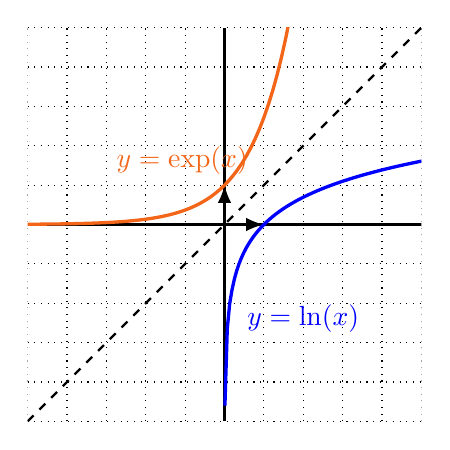
\begin{tikzpicture}[scale=0.5]
\clip (-5,-5) rectangle (5,5);
\draw [thin, dotted] (-5,-5) grid (5,5);
\draw [thick] (-5,0)--(7,0);
\draw [thick] (0,-5) -- (0,5);
\draw [very thick,->,>=latex] (0,0)--(0,1);
\draw [very thick,->,>=latex] (0,0)--(1,0);
\draw [very thick, ocre,domain=-5:6,samples=100] plot (\x,{exp(\x)});
\draw [very thick, blue,domain=0.01:6,samples=100] plot (\x,{ln(\x)});
\draw [ thick, dashed,domain=-5:6,samples=100] plot (\x,{\x});
\draw [thick,ocre] (-3,1) node[above right] {$y=\exp(x)$};
\draw [thick, blue] (2,-3) node[above] {$y=\ln(x)$};
\end{tikzpicture}
\end{center}

Cette propriété est vraie pour toutes les fonctions réciproques l'une de l'autre. Par exemple, vous pouvez observer le même phénomène en regardant les courbes des fonctions $x\mapsto x^2$ et $x\mapsto \sqrt{x}$ sur $[0;+\infty[$. Autre exemple, la fonction inverse, qui est sa propre réciproque. La courbe de cette fonction est elle-même symétrique par rapport à la droite d'équation $y=x$.




\end{document}